%=======================================================================
%
% ------------------------------------------------------------------------
% ------------------------------------------------------------------------
% abnTeX2: Modelo de Trabalho Academico  em conformidade com 
% ABNT NBR 14724:2011: Informacao e documentacao - Trabalhos academicos
% ------------------------------------------------------------------------
%Customização Unoesc
% ------------------------------------------------------------------------
% Autor:  Jonas Alessi(alessi.jonas@gmail.com
% Versão: 10 de Julho 2013.
% Edição: TexStudio
% Codificação: UTF-8
% LaTeX:  abnTeX2
%
%=======================================================================

\documentclass[
	% -- opções da classe memoir --
	12pt,				% tamanho da fonte	
	oneside,          % não imprimir em verso e anverso, oposto do twoside 
	a4paper,			% tamanho do papel. 
	% -- opções da classe abntex2 --
	chapter=TITLE,		% títulos de capítulos convertidos em letras maiúsculas
	section=TITLE,		% títulos de seções convertidos em letras maiúsculas
	subsection=TITLE,	% títulos de subseções convertidos em letras maiúsculas
	%subsubsection=TITLE,% títulos de subsubseções convertidos em letras maiúsculas
	% -- opções do pacote babel --
	english,			% idioma adicional para hifenização
	brazil			% o último idioma é o principal do documento
	,sumario=tradicional
	]{abntex2-unoesc}
	
	\usepackage{xcolor}
	% Definindo novas cores
	\definecolor{verde}{rgb}{0,0.5,0}
	% Configurando layout para mostrar codigos C++
	\usepackage{listings}
	\lstset{
		language=C++,
		basicstyle=\ttfamily\small, 
		keywordstyle=\color{blue}, 
		stringstyle=\color{verde}, 
		commentstyle=\color{red}, 
		extendedchars=true, 
		showspaces=false, 
		showstringspaces=false, 
		numbers=left,
		numberstyle=\tiny,
		breaklines=true, 
		backgroundcolor=\color{green!10},
		breakautoindent=true, 
		captionpos=b,
		xleftmargin=0pt,
	}
	\pagestyle{empty}
	


% ---
% Pacotes fundamentais 
% ---
\usepackage{cmap}				% Mapear caracteres especiais no PDF
\usepackage{times}			    % Usa a fonte Latin Modern			
\usepackage[T1]{fontenc}		% Selecao de codigos de fonte.
\usepackage[utf8]{inputenc}		% Codificacao do documento (conversão automática dos acentos)
\usepackage{lastpage}			% Usado pela Ficha catalográfica
\usepackage{indentfirst}		% Indenta o primeiro parágrafo de cada seção.
\usepackage{color}				% Controle das cores
\usepackage{graphicx}			% Inclusão de gráficos
\usepackage{amsfonts}			% Símbolos
%----Ajuste no alinhamento das listas
\usepackage{enumitem}
\setitemize[0]{itemindent=0.4cm,itemsep=0pt}
\setenumerate[0]{itemindent=0.5cm,itemsep=0pt}
%------
% ---
% Pacotes de citações
% ---
\usepackage[brazilian,hyperpageref]{backref}	 					  % Paginas com as citações na bibl

%Referência
\usepackage[alf, 	
			 		abnt-emphasize=bf,
				    abnt-url-package=none,
				    abnt-repeated-title-omit=yes,
				    abnt-full-initials=yes,                                        %yes nome por extenso, no apenas iniciais
					abnt-etal-list=3												%abreviar com mais de 3 autores
]{abntex2/abntex2cite}				 														    % Citações padrão ABNT
\usepackage{lipsum}							   								       % para geração de dummy text

%\captionsetup[table]{justification=raggedright}
% Configurações de aparência do PDF final
% alterando o aspecto da cor azul
\definecolor{blue}{RGB}{41,5,195}

% --- 
% Espaçamentos entre linhas e parágrafos 
% --- 
% O tamanho do parágrafo é dado por:
\setlength{\parindent}{1.25cm}
\linespread{1.5}

%Espaçamento depois dos títulos
\setlength{\afterchapskip}{\baselineskip}
% %\setlength{\afterchapskip}{\lineskip}

% Controle do espaçamento entre um parágrafo e outro:
\setlength{\parskip}{0cm}  % tente também \onelineskip

\hangcaption
\captionstyle[\raggedright]{}

%Estava mostrando nas referencias quais paginas estavam sendo referenciadas
\renewcommand{\backref}{}
\renewcommand*{\backrefalt}[4]{}

%Reduzir a fonte do caption
\captionnamefont{\ABNTEXfontereduzida}
\captiontitlefont{\ABNTEXfontereduzida}
%Ajuste nas listas de tabela, ilustrações e quadros
\setlength\cftbeforechapterskip{0pt}
% ---
% compila o indice
% ---
\makeindex
% ---

\lstdefinestyle{CPP}
{
	language=C++,
	alsolanguage={[Sharp]C},
	basicstyle=\ttfamily\small, 
	keywordstyle=\color{blue}, 
	stringstyle=\color{green}, 
	commentstyle=\color{red}, 
	extendedchars=true, 
	showspaces=false, 
	showstringspaces=false, 
	numbers=left,
	numberstyle=\tiny,
	breaklines=true, 
	backgroundcolor=\color{green!10},
	breakautoindent=true, 
	captionpos=b,
	xleftmargin=0pt,
}
	\usepackage{lscape}

%----Include da capa é fora do documento 
% ---
% Informações de dados para CAPA e FOLHA DE ROSTO
% ---
\titulo{TRABALHO FINAL DE INSTRUMENTAÇÃO E PROCESSAMENTO DE SINAIS}
\autor{\tiny ARTHUR BOESING BILIBIO\\
	EDUARDA ISSLER BARBIERI\\
	JOHNATAN MARCEL DA ROSA\\
	PATRÍCIA COMUNELLO\\
	WAGNER CASAGRANDE\\
	}
\local{Joaçaba}
\data{2017}
\orientador{MSc. Geovani Rodrigo Scolaro}
\instituicao{UNIVERSIDADE DO OESTE DE SANTA CATARINA}
\tipotrabalho{Tese (Doutorado)}
% O preambulo deve conter o tipo do trabalho, o objetivo, 
% o nome da instituição e a área de concentração 
\preambulo{Trabalho de apresentação ao Curso de Engenharia de Computação, Área das Ciências Exatas e da Terra, da Universidade do Oeste de Santa Catarina, como requisito à obtenção de nota na disciplina de Instrumentação e Processamento de Sinais.}
% ---

%---

\begin{document}
% Retira espaço extra obsoleto entre as frases.
\frenchspacing 

% ----------------------------------------------------------
% ELEMENTOS PRÉ-TEXTUAIS
% ----------------------------------------------------------

%--- CAPA ----
\imprimircapa

% --- FOLHA DE ROSTO
%\imprimirfolhaderosto
% \imprimirfolhaderosto* (o * indica que haverá a ficha bibliográfica)

% Inserir FOLHA DE APROVAÇÃO
%\begin{folhadeaprovacao}

  \begin{center}
  \vspace*{-1.2cm}
    {\large\imprimirautor}

    \vspace*{\fill}
    {\large\imprimirtitulo}
    \vspace*{\fill}
    
    \hspace{.45\textwidth}
    \begin{minipage}{.5\textwidth}
        \imprimirpreambulo
    \end{minipage}%
    \vspace*{\fill}
   \end{center}
    
  \begin{flushleft}
  	 Aprovado em:\underline{\hspace{1cm}}/\underline{\hspace{1cm}}/\underline{\hspace{1.2cm}}
  \end{flushleft}
  \begin{center}
  BANCA EXAMINADORA
  \end{center}

   \assinatura{\imprimirorientador \\ 
   					   Universidade do Oeste de Santa Catarina\\
   					    Nota atribuída \underline{\hspace{1.1cm}}
   } 
   \assinatura{Professor \\ 
   					   Universidade do Oeste de Santa Catarina\\
   					    Nota atribuída \underline{\hspace{1.1cm}}
   }
    \assinatura{Professor \\ 
   					   Universidade do Oeste de Santa Catarina\\
   					    Nota atribuída \underline{\hspace{1.1cm}}
    }
      
%   \begin{center}
    \vspace*{3cm}
%    {\large\imprimirlocal}
%    \par
%    {\textbf{\large\imprimirdata}}
%    \vspace*{1cm}
%  \end{center}
  
\end{folhadeaprovacao}

%% DEDICATÓRIA
%\begin{dedicatoria}
 \vspace*{\fill}
 \noindent
  \raggedleft
 \begin{minipage}{.54\textwidth}
    Dedico este trabalho a meus pais, fonte de meus conhecimentos  e saber. Graças a eles, tornei-me uma pessoa capaz de lutar para que meus sonhos e objetivos fossem sempre alcançados, sem jamais desanimar. Considero-me forte porque eles me ensinaram a ser forte.
   \end{minipage}
\end{dedicatoria}


%% AGRADECIMENTO
%\begin{agradecimentos}

\lipsum[1-1]


\end{agradecimentos}

%%EPÍGRAFE
%\begin{epigrafe}
    \vspace*{\fill}
	\begin{flushright}
		Não vos amoldeis às estruturas deste mundo, \\
		mas transformai-vos pela renovação da mente, \\
		a fim de distinguir qual é a vontade de Deus: \\
		o que é bom, o que Lhe é agradável, o que é perfeito.\\
		(Bíblia Sagrada, Romanos 12, 2)
	\end{flushright}
\end{epigrafe}

% RESUMO
%
% resumo em português
\begin{resumo}
\noindent
A Inteligência Artificial pode ser caracterizada como sendo um estudo de novos dispositivos computacionais ou de novos métodos para resolução de problemas, afim de imitar ou reproduzir um comportamento inteligente. O objetivo deste trabalho é implementar um sistema inteligente que contenha dois agentes autônomos, que se locomovam em um circuito pré-determinado e realizem o controle de velocidade e distância entre si. O sistema deve ser composto por um software supervisório que seja capaz de apresentar os parâmetros de configuração e monitoramento dos agentes em tempo real, mostrando velocidade e distância entre eles, possibilitando dessa forma, a avaliação do sistema. Para o desenvolvimento deste trabalho foi necessário criar o protótipo dos agentes seguidores de linha, desenvolver o firmware para seguir linha, para controle de distância e velocidade, também foi necessário criar um software supervisório para monitoramento e configuração dos agentes. 
Este trabalho tem como requisito à obtenção de nota na disciplina de Inteligência Artificial II, onde as aulas foram dedicadas para o desenvolvimento do mesmo. Como metodologia adotada, o projeto foi divido em equipes devido grande número de acadêmicos.


 \vspace{0.2cm}
    
 
 Palavras-chave: Inteligência Artificial. Sistema Inteligente. Firmware. Supervisório. 
\end{resumo}

% resumo em inglês
\begin{resumo}[Abstract]	
 	\begin{otherlanguage*}{english}
 	\noindent 
	\textit{
	The Artificial Intelligence can be characterized as being hum new study computational devices or new methods problem resolution in order to imitate or play hum intelligent behavior.
	The objective this work and implement intelligent hum system containing two autonomous agents, which to move about in pre-hum determined circuit and realize the speed control and distance between them. The system must be composed of a monitoring software to be able to display the configuration parameters and monitoring of agents in real time, displaying speed and distance between they, enabling thus, the evaluation system.
	For work this development was necessary to create the prototype of line followers agents, develop firmware to follow you Line, control distance and speed, also it was necessary to create a monitoring software paragraph monitoring and configuration of agents.
	This has work as requirement to note obtaining the Artificial Intelligence II discipline, where were the lessons dedicated to the development do same. As methodology adopted, the project was divided into teams due grande number of academic.
	}
   \vspace{0.2cm}
 
\textit{
    Key-words: Artificial Intelligence. Intelligent System. Firmware. Supervisory.	
}
 	\end{otherlanguage*}
\end{resumo}

% lista de ilustrações
\pdfbookmark[0]{\listfigurename}{lof}
\listoffigures*
\cleardoublepage
% ---

% lista de quadros
% --- 
%PRECISO VER COMO FAZER O CONTROLE DE QUANDO TIVER MENOS Q 10 VAI PARA LISTA DE ILUSTRAÇÕES
\pdfbookmark[0]{\listofquadrosname}{loq}
%\listofquadros*
\cleardoublepage
% ---

% LISTA DE TABELAS
\pdfbookmark[0]{\listtablename}{lot}
\listoftables*
\cleardoublepage  %-- força proxima pagina

% ---
% inserir lista de abreviaturas e siglas
% ---
%\begin{siglas}
%  \item[IA] Inteligência Artificial
%  \item[CC] Corrente Contínua
%  \item[FHSS] Frequency Hopping Spread Spectrum
%  \item[IR] Infravermelho
%  \item[ISM] Industrial, Scientific and Medicine
%  \item[LDR] Light Dependent Resistor
%  \item[LED] Light Emitting Diode
% \item[MLP] Perceptron Multi-Camadas  
%  \item[PAN] Personal Area Network
%\item[PWM] Pulse Width Modulation
%\item[XP] Extreme Programming
%\end{siglas}
% ---

% ---
% inserir lista de símbolos
% ---

% ---

% SUMARIO
\pdfbookmark[0]{\contentsname}{toc}
\tableofcontents*
\cleardoublepage

% ------------------------------------------------------
% ELEMENTOS TEXTUAIS
% ------------------------------------------------------
\textual
% INTRODUÇÃO
% ----------------------------------------------------------
% Introdução
%Ex: \chapter{TÍTULO A SER IMPRESSO NO CORPO DO TEXTO}{Título no cabeçalho}{Título no Sumario}
% ----------------------------------------------------------
\chapter{INTRODUÇÃO} 
Diariamente nos deparamos com sinais que contém informações sobre algum fenômeno ou acontecimento. Tais sinais precisam ser manipulados e processados para que se tornem utilizáveis, deste modo, foram aplicados os conhecimentos adquiridos na disciplina de instrumentação e processamento de sinais para desenvolver um sistema capaz de gerar sinais com auxílio do gerador de função, para posteriormente filtrá-los e amplificá-los em hardware, possibilitando visualização e análise em software.


\chapter{DESCRIÇÃO DO PROJETO}
Este trabalho propõe o desenvolvimento de um sistema microcontrolado para aquisição e processamento de sinais.

\section{OBJETIVO GERAL}
Implementar um sistema microcontrolado de aquisição para qualquer tipo de sinal utilizando uma frequência de amostragem de 200 Hz. Apresentando toda a instrumentação necessária para a correta visualização em software, dos sinais gerados pelo gerador de função.

\section{OBJETIVOS ESPECÍFICOS}
Como objetivos específicos, destacamos:
 \begin{itemize}
 	\item Projetar circuito elétrico dos filtros e amplificador.
  	\item Esquematizar circuito elétrico do hardware completo.
 	\item Confeccionar hardware do sistema.
 	\item Desenvolver o firmware para processamento e conversão do sinal.
 	\item Desenvolver o software supervisório para visualização e manipulação do sinal.
 	\item Realizar a documentação do projeto.
 \end{itemize}

\chapter{METODOLOGIA}
Este projeto foi executado durante as aulas da disciplina de Instrumentação e Processamento de sinais, onde o grupo foi dividido em equipes de trabalhos, podemos verificar a divisão na Tabela 1. Para a elaboração, foram realizadas pesquisas, seguido do estudo de caso para desenvolvimento do protótipo, tutoriais e vídeos informativos através de pesquisa eletrônica.  
\begin{table}[htb]
	\IBGEtab{ %Este macro alinha o titulo e fonte a esquerda \IBGEtab{caption label} {tabela ou figura} {fonte}
		\caption{Equipes de trabalho}
		\label{tab:esquerda}
	}{
	\begin{tabular}{p{8.3cm}lp{8cm}}
		\hline
		\textbf{Atividades}                      & \textbf{Equipes de trabalho} \\ \hline
		Esquemático do circuito elétrico                        & Eduarda e Patrícia\\ \hline
		Desenvolvimento do hardware do sistema   & Eduarda e Wagner\\  \hline
		Desenvolvimento do firmware              & Johnatan e Wagner \\  \hline
		Desenvolvimento do software supervisório & Arthur\\  \hline
		Documentação do projeto                  & Eduarda e Patrícia\\  \hline
	\end{tabular}
}{
\fonte{os autores.}
%  \nota{Exemplo de nota}
% \nota[Anotações]{Exemplo nota personalizada}
}
\end{table}


%%FUNDAMENTAÇÃO TEÓRICA
%\chapter{FUNDAMENTAÇÃO TEÓRICA}

\textcolor{red}{Apresentar estudos que contemple a temática abordada. Respeitar a autoria,
nas citações diretas e indiretas. Evitar parágrafos muito longos. Evitar seções e
subseções muito curtas.}

\section{Exemplo de Seção}

\subsection{Exemplo subSeção}

\subsubsection{Exemplo subsubsection}

% FALTA AJUSTAR \subsubsubsection{Exemplo subsubsubsection}

%DESENVOLVIMENTO
\chapter{DESENVOLVIMENTO}
Nesta seção, será descrito em detalhes cada etapa do desenvolvimento do sistema de aquisição e processamento de sinais. 

Com finalidade de detalhar o funcionamento, podemos observar na Figura 1, o fluxo seguido pelo sistema desenvolvido.

\begin{figure}[h] 
	\begin{center} 
		\begin{center}
			\changecaptionwidth 
			\captionwidth{15.6cm} %posicionamento da legenda
			\caption{\label{fig_fot7}Fluxo do sistema de aquisição e processamento do sinal.}
			\fbox{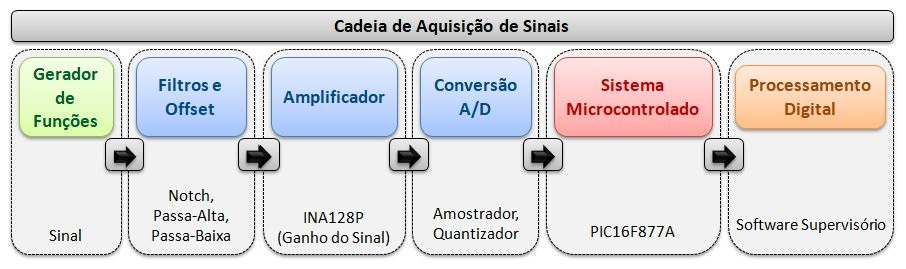
\includegraphics[scale=0.80]{figuras/fluxograma}}
			\fonte{adaptado de \cite{Geovani1}.}
		\end{center}
	\end{center}
\end{figure} 

 

\section{FILTROS ATIVOS}
O sinal é gerado com auxílio do gerador de funções, que inicia o processo passando pelo sistema de filtragem. Utilizando a Equação 4.1, calculou-se a frequência de corte dos filtros, possibilitando a escolha correta dos resistores e capacitores \cite{Geovani3}.

\begin{equation}
	fc = \frac {1}{2 \times \pi \times R \times C}
\end{equation}

Onde:
\begin{itemize}
	\item \textit{fc}: frequência de corte;
	\item \textit{R}: resistência ($\Omega$);
	\item \textit{C}: Capacitância (F).
\end{itemize}
 
Para o sistema de filtragem foi utilizado um filtro passa altas com frequência de corte em 0.5 Hz e um passa baixas com frequência de corte em 90 Hz. Aplicando a equação citada acima, os componentes resultantes para que os filtros funcionassem corretamente, podem ser visualizados no esquemático do circuito elétrico na Figura 2.

\begin{figure}[h] 
	\begin{center} 
		\begin{center}
			\changecaptionwidth 
			\captionwidth{15.8cm} %posicionamento da legenda
			\caption{\label{fig_fot7}Esquemático do circuito elétrico dos filtros do sinal}
			\fbox{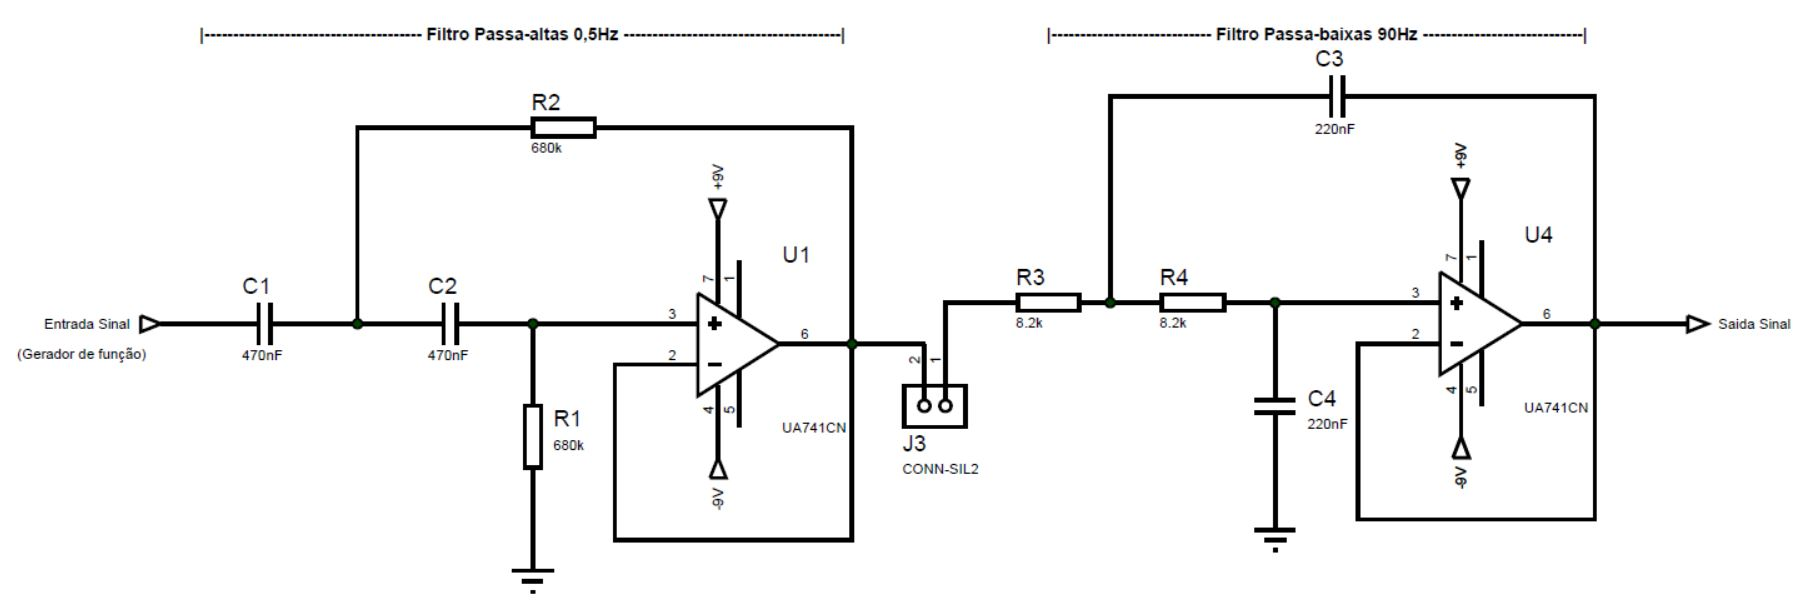
\includegraphics[scale=0.41]{figuras/circuitoFiltro}}
			\fonte{os autores.}
		\end{center}
	\end{center}
\end{figure} 

\section{AMPLIFICADOR}
Posteriormente à filtragem, para ser utilizado o sinal necessita ser amplificado. Diante isso, foi feito uso do amplificador de instrumentação INA128P. Neste componente, o valor de saída é definido pelo resistor de ganho, que é ligado aos pinos 1 e 8. Foi utilizado no desenvolvimento um resistor de 5.6k, obtendo uma amplificação de 10 vezes, de acordo com a fórmula de ganho apresentada na Equação 4.2 \cite{Geovani2}.  
\begin{equation}
	G = 1 + \frac {50k\Omega}{R_G}
\end{equation}

Onde:

\textit{G}: ganho;

\textit{R\tiny{G}}: resistor de ganho ($\Omega$).

A Figura 2 apresenta o circuito do amplificador. Onde R5 é o resistor de ganho, C5 e C6 são capacitores de 100nF para estabilizar a fonte do microcontrolador para não oscilar.
\newpage
\begin{figure}[h] 
	\begin{center} 
		\begin{center}
			\changecaptionwidth 
			\captionwidth{11.0cm} %posicionamento da legenda
			\caption{\label{fig_fot7}Esquemático do circuito elétrico do amplificador do sinal}
			\fbox{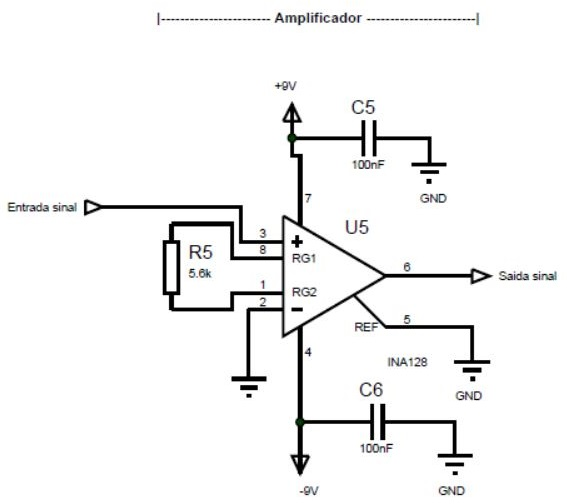
\includegraphics[scale=0.90]{figuras/circuitoAmplificador}}
			\fonte{os autores.}
		\end{center}
	\end{center}
\end{figure} 


\section{FIRMWARE}
Após filtrado e amplificado, o sinal precisa ser convertido de analógico para digital, este processo foi realizado com a utilização de um microcontrolador PIC 16F877A, pois possui um conversos A/D interno, tornando o processo simples. A Figura 4, demonstra o esquemático do circuito elétrico desenvolvido para tal processo. 

\begin{figure}[htb]
	\caption{Esquemático do circuito elétrico do sistema de conversão A/D}
	%	\label{diag:grafico6}
	\borda{
		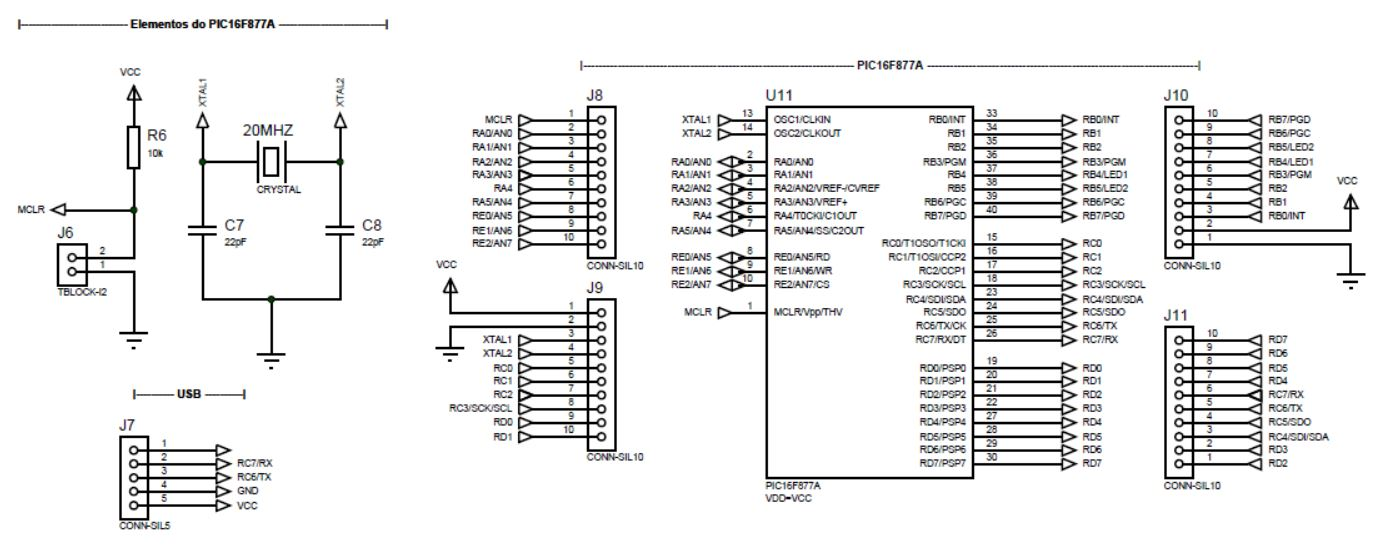
\includegraphics[scale=0.52]{figuras/circuitoPIC}
	}
	\fonte{os autores.}
\end{figure}

Posteriormente a conversão A/D do sinal, o mesmo é formatado com a utilização de colchetes para ser enviado so software supervisório. A leitura do sinal ocorre a cada 5 ms, onde são coletadas 200 amostras a cada período de leitura.

O código fonte do firmware pode ser consultado no Apêndice A.

\section{SOFTWARE}
Para o desenvolvimento do software supervisório, foi utilizado o software Qt Creator. A Figura 5, demonstra a tela inicial, que faz a leitura dos dados, através do botão "Ler Dados", no botão "Apresentar Gráfico" é possível visualizar a entrada do sinal, bem como manipulá-lo através do botão "Calcular DFT" e "Apresentar DFT".  Fazendo o uso de um período de mil amostras, é possível analisar o sinal através de uma DFT (Discrete Fourier Transform). 

\begin{figure}[htb]
	\caption{Software supervisório}
	%	\label{diag:grafico6}
	\borda{
		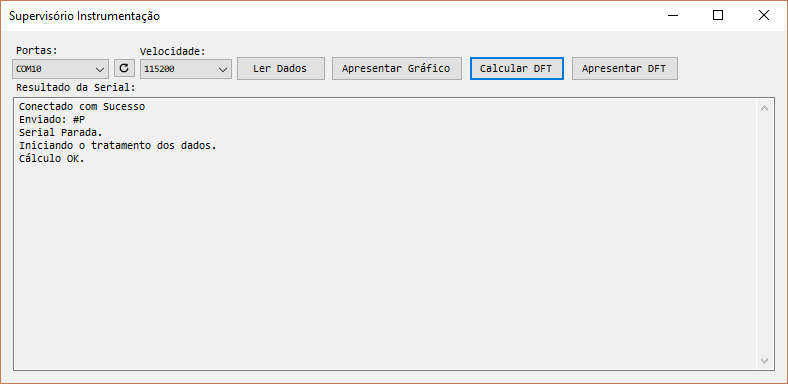
\includegraphics[scale=0.54]{figuras/software}
	}
	\fonte{os autores.}
\end{figure}

O código fonte de software supervisório desenvolvido pode ser verificado no Apêndice B.

\section{SISTEMA DE INSTRUMENTAÇÃO E PROCESSAMENTO DE SINAIS}
Após o detalhamento de cada módulo comentado nas seções anteriores, a Figura 6 demonstra o esquemático completo do hardware.

\begin{figure}[htb]
	\caption{Esquemático do circuito elétrico do sistema de instrumentação e processamento de sinais}
	%	\label{diag:grafico6}
	\borda{
		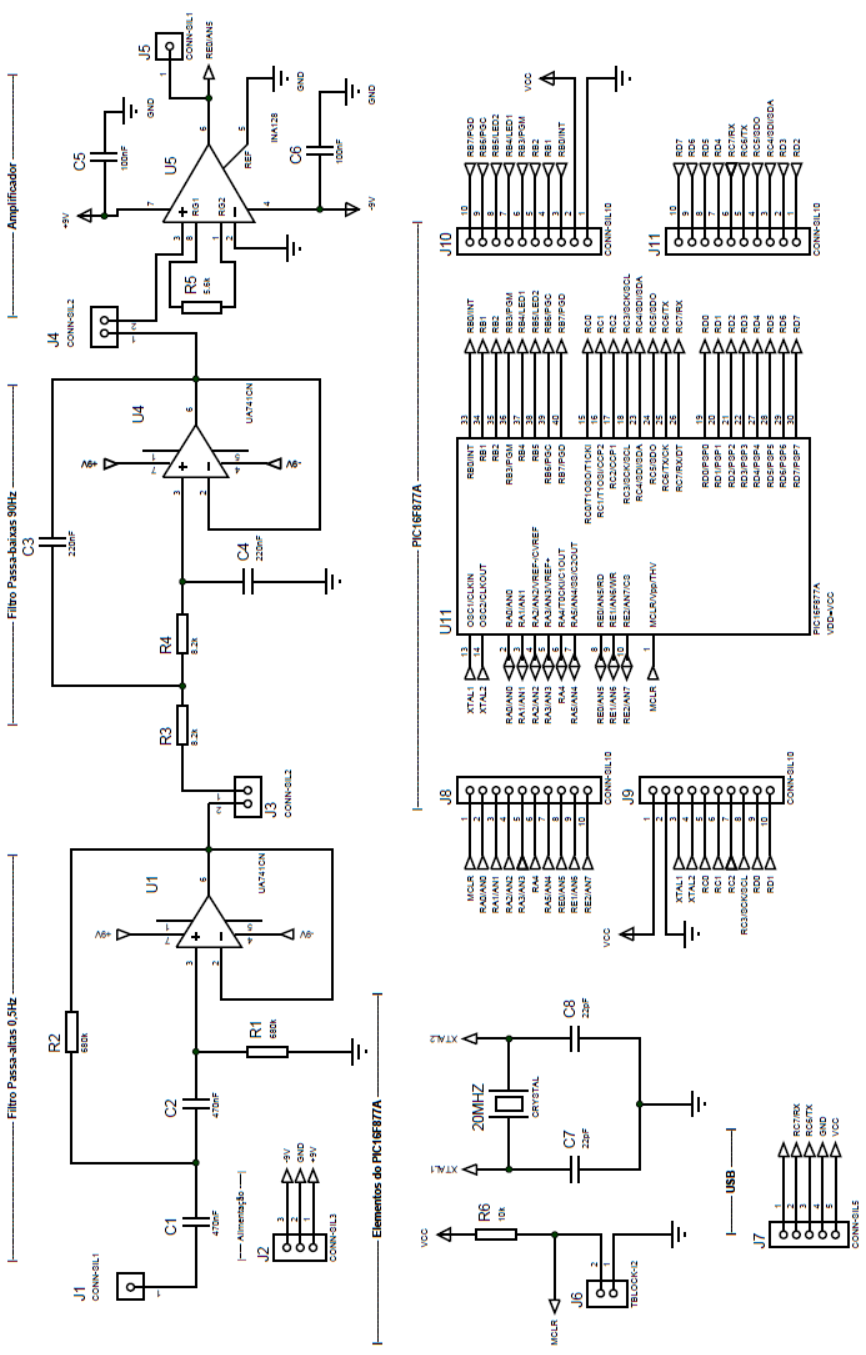
\includegraphics[scale=0.83]{figuras/completo}
	}
	\fonte{os autores.}
\end{figure}


%RESULTADOS
\chapter{RESULTADOS}
Foram realizados testes simulando frequências com o gerador de função. Foi simulado uma frequência de 37 Hz, que passou pelos filtros e amplificador, posteriormente processado pelo microcontrolador e enviado ao software, podemos visualizar o sinal na Figura 7 e a Figura 8 demonstra o sinal manipulado com o uso da DFT.

\begin{figure}[htb]
	\caption{Software supervisório - Entrada sinal}
	%	\label{diag:grafico6}
	\borda{
		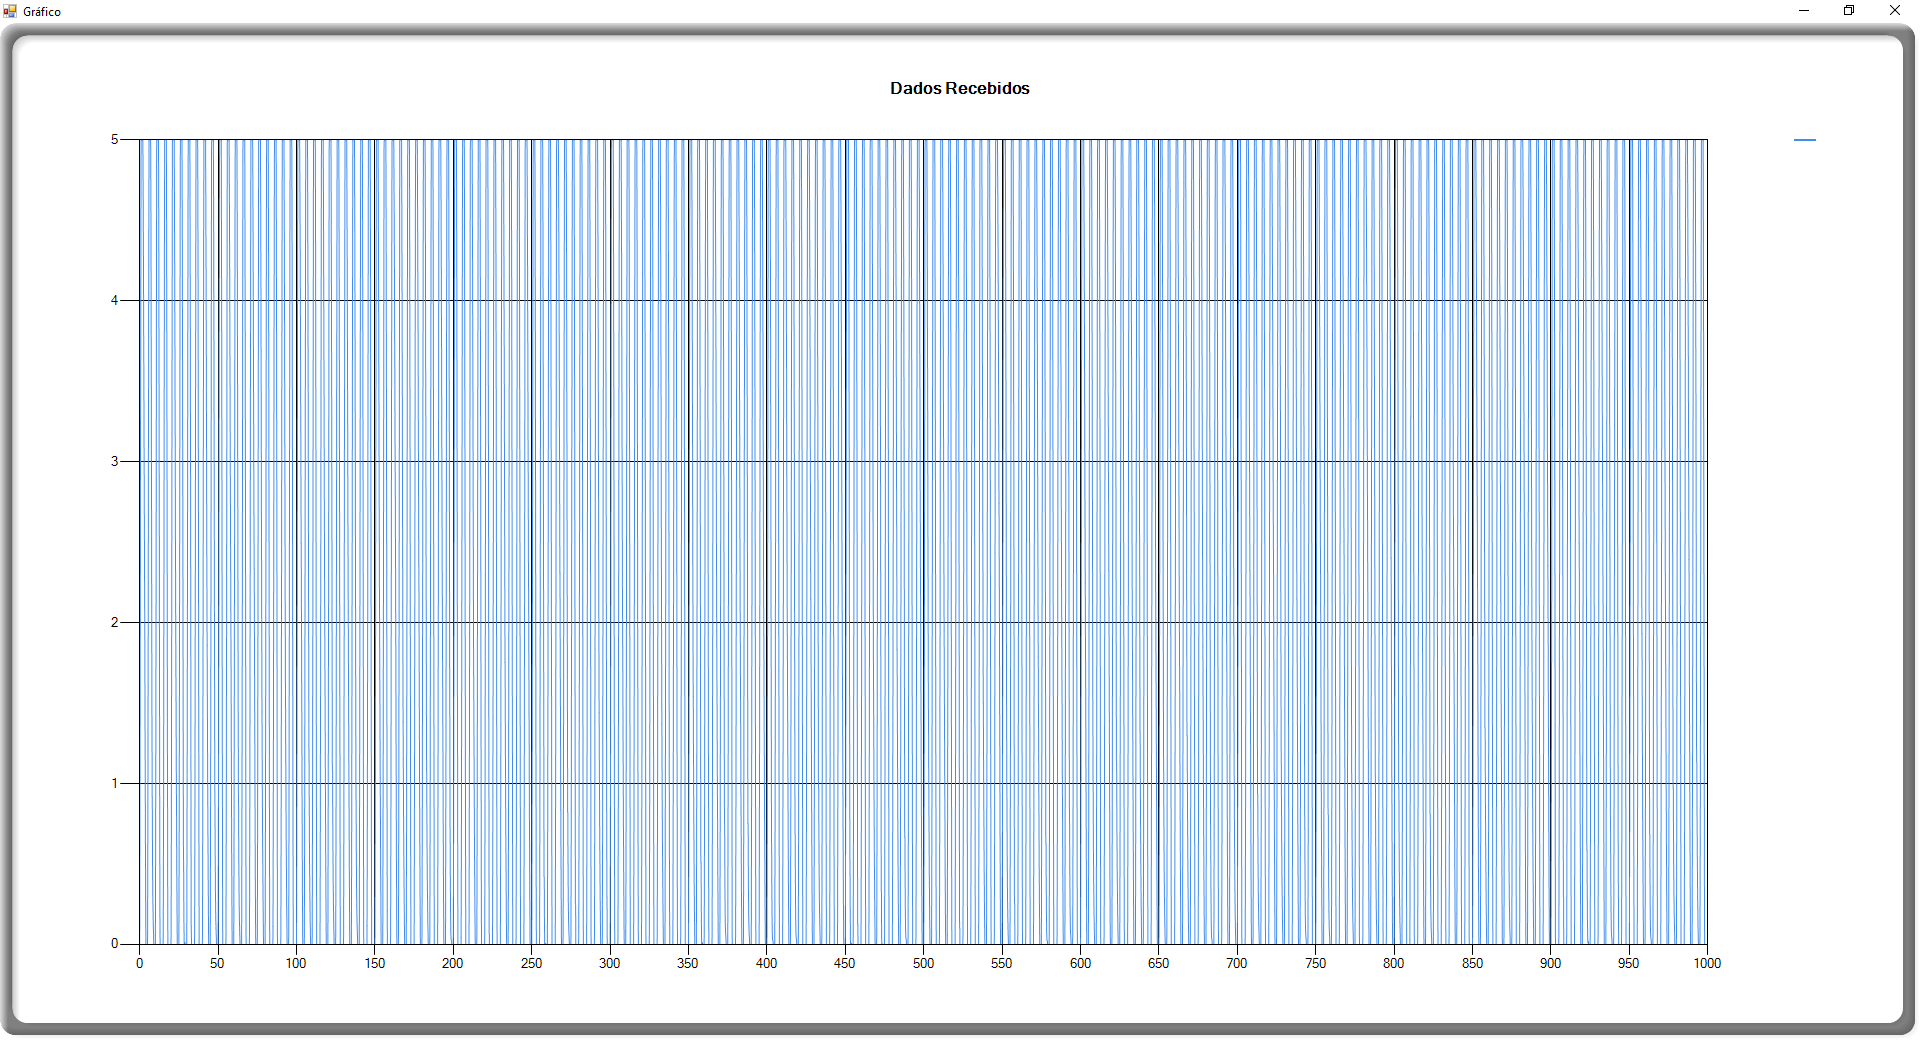
\includegraphics[scale=0.22]{figuras/sinal37}
	}
	\fonte{os autores.}
\end{figure}

\begin{figure}[htb]
	\caption{Software supervisório - Aplicado DFT}
	%	\label{diag:grafico6}
	\borda{
		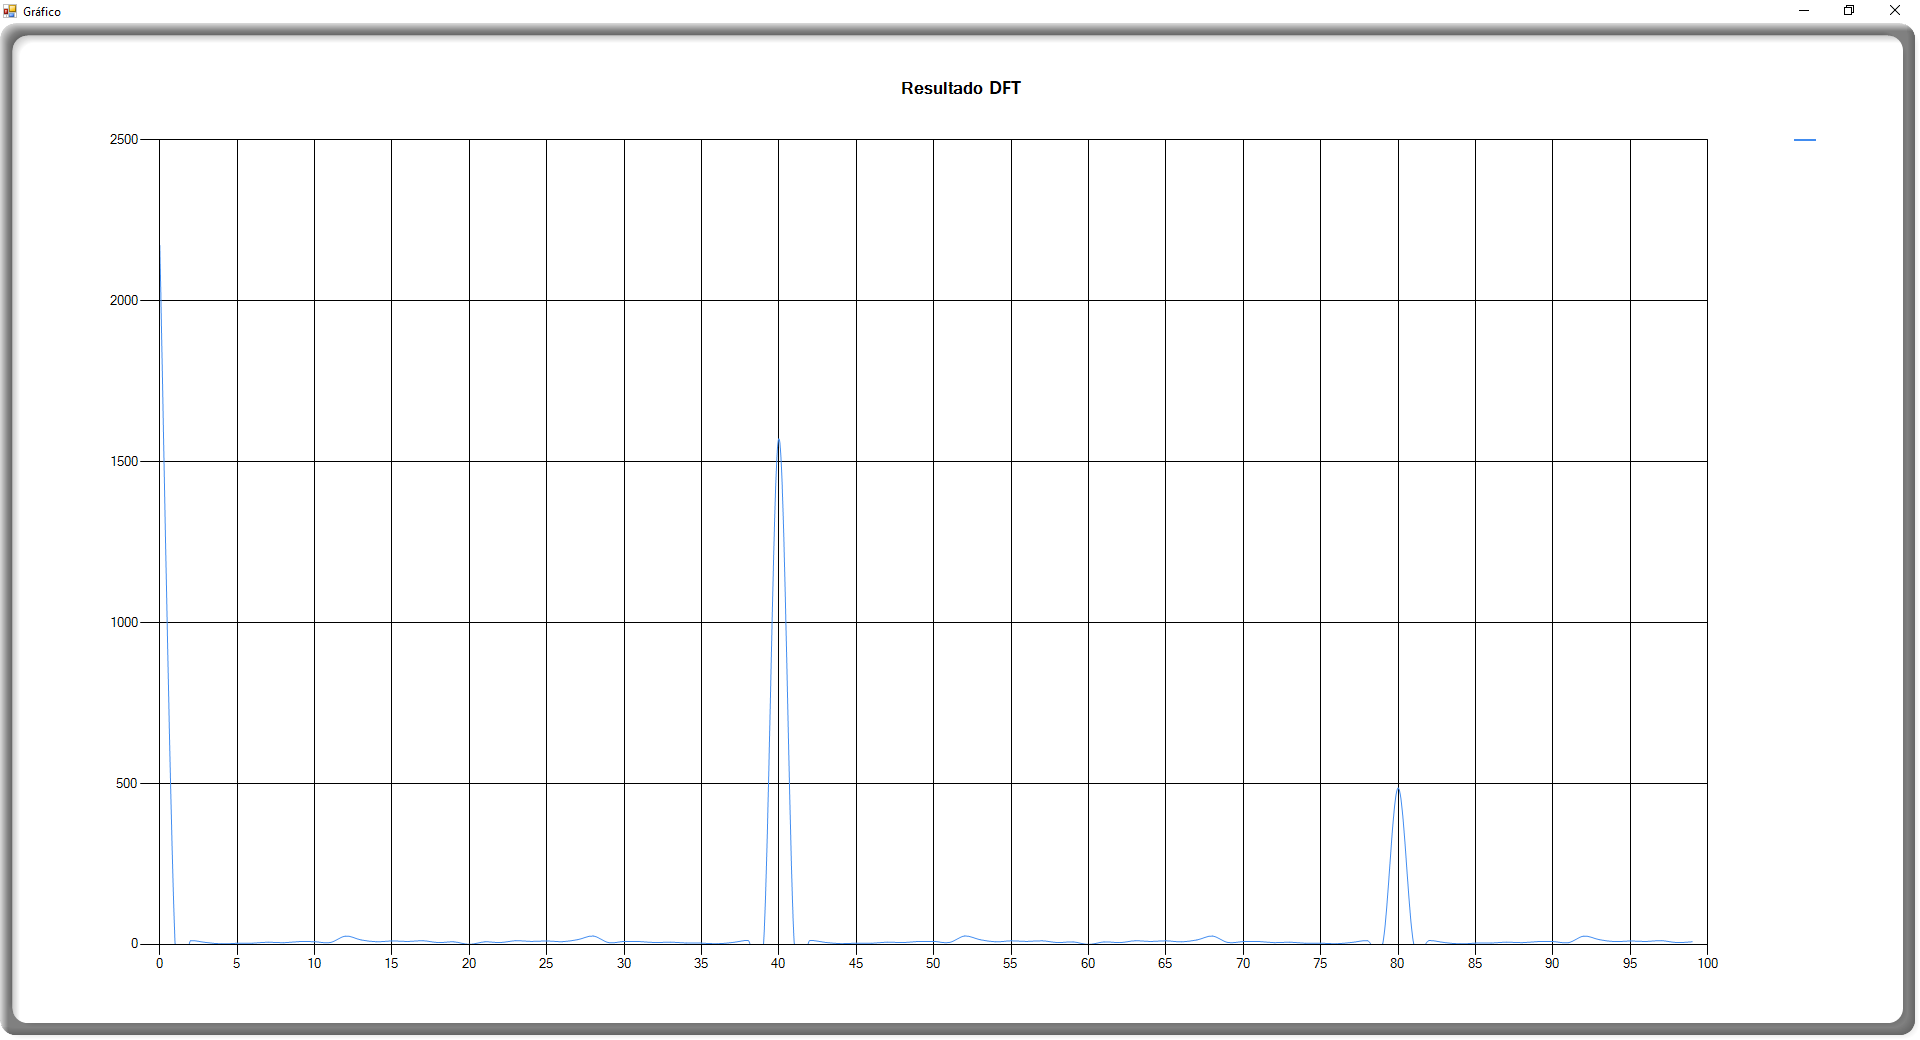
\includegraphics[scale=0.37]{figuras/dft37}
	}
	\fonte{os autores.}
\end{figure}

No segundo teste foi utilizado uma frequência de 67 Hz, podemos visualizar a leitura do sinal na Figura 9 e a DFT na Figura 10.

\begin{figure}[htb]
	\caption{Software supervisório - Entrada sinal}
	%	\label{diag:grafico6}
	\borda{
		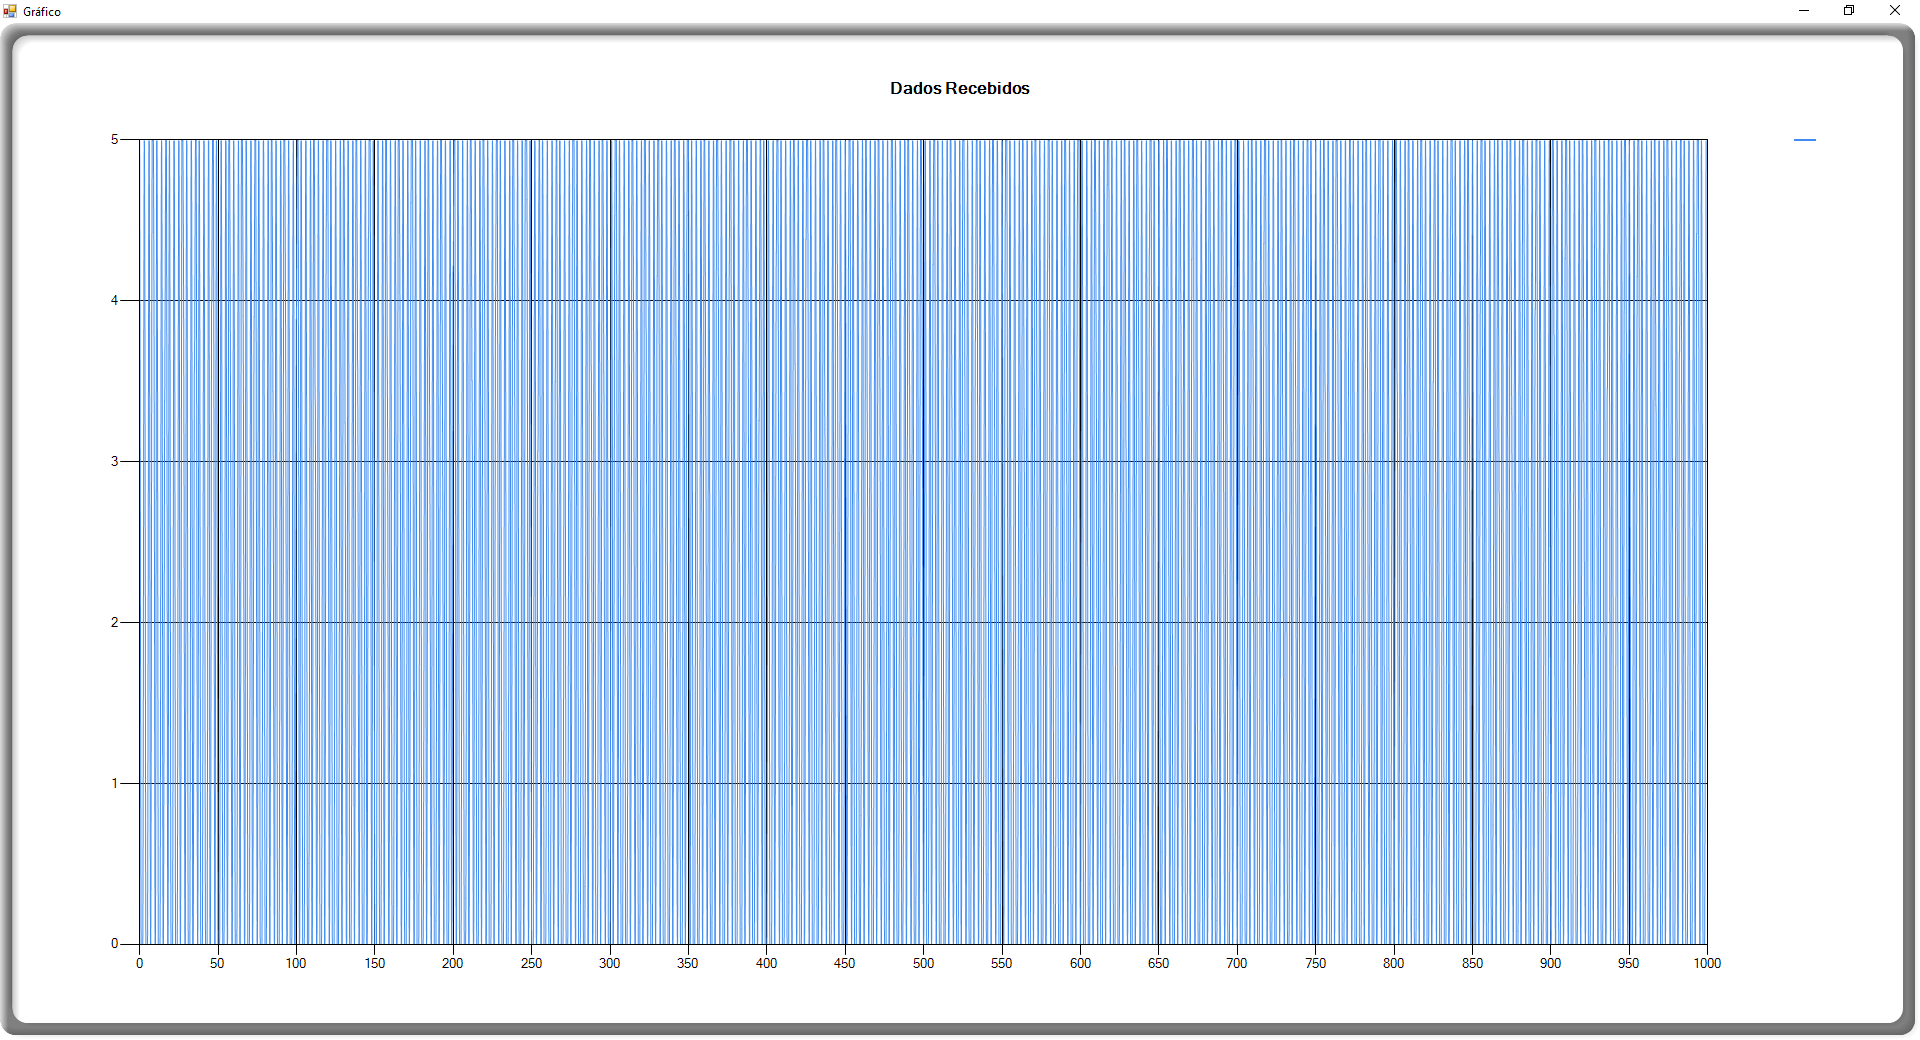
\includegraphics[scale=0.22]{figuras/sinal67}
	}
	\fonte{os autores.}
\end{figure}

\begin{figure}[htb]
	\caption{Software supervisório - Aplicado DFT}
	%	\label{diag:grafico6}
	\borda{
		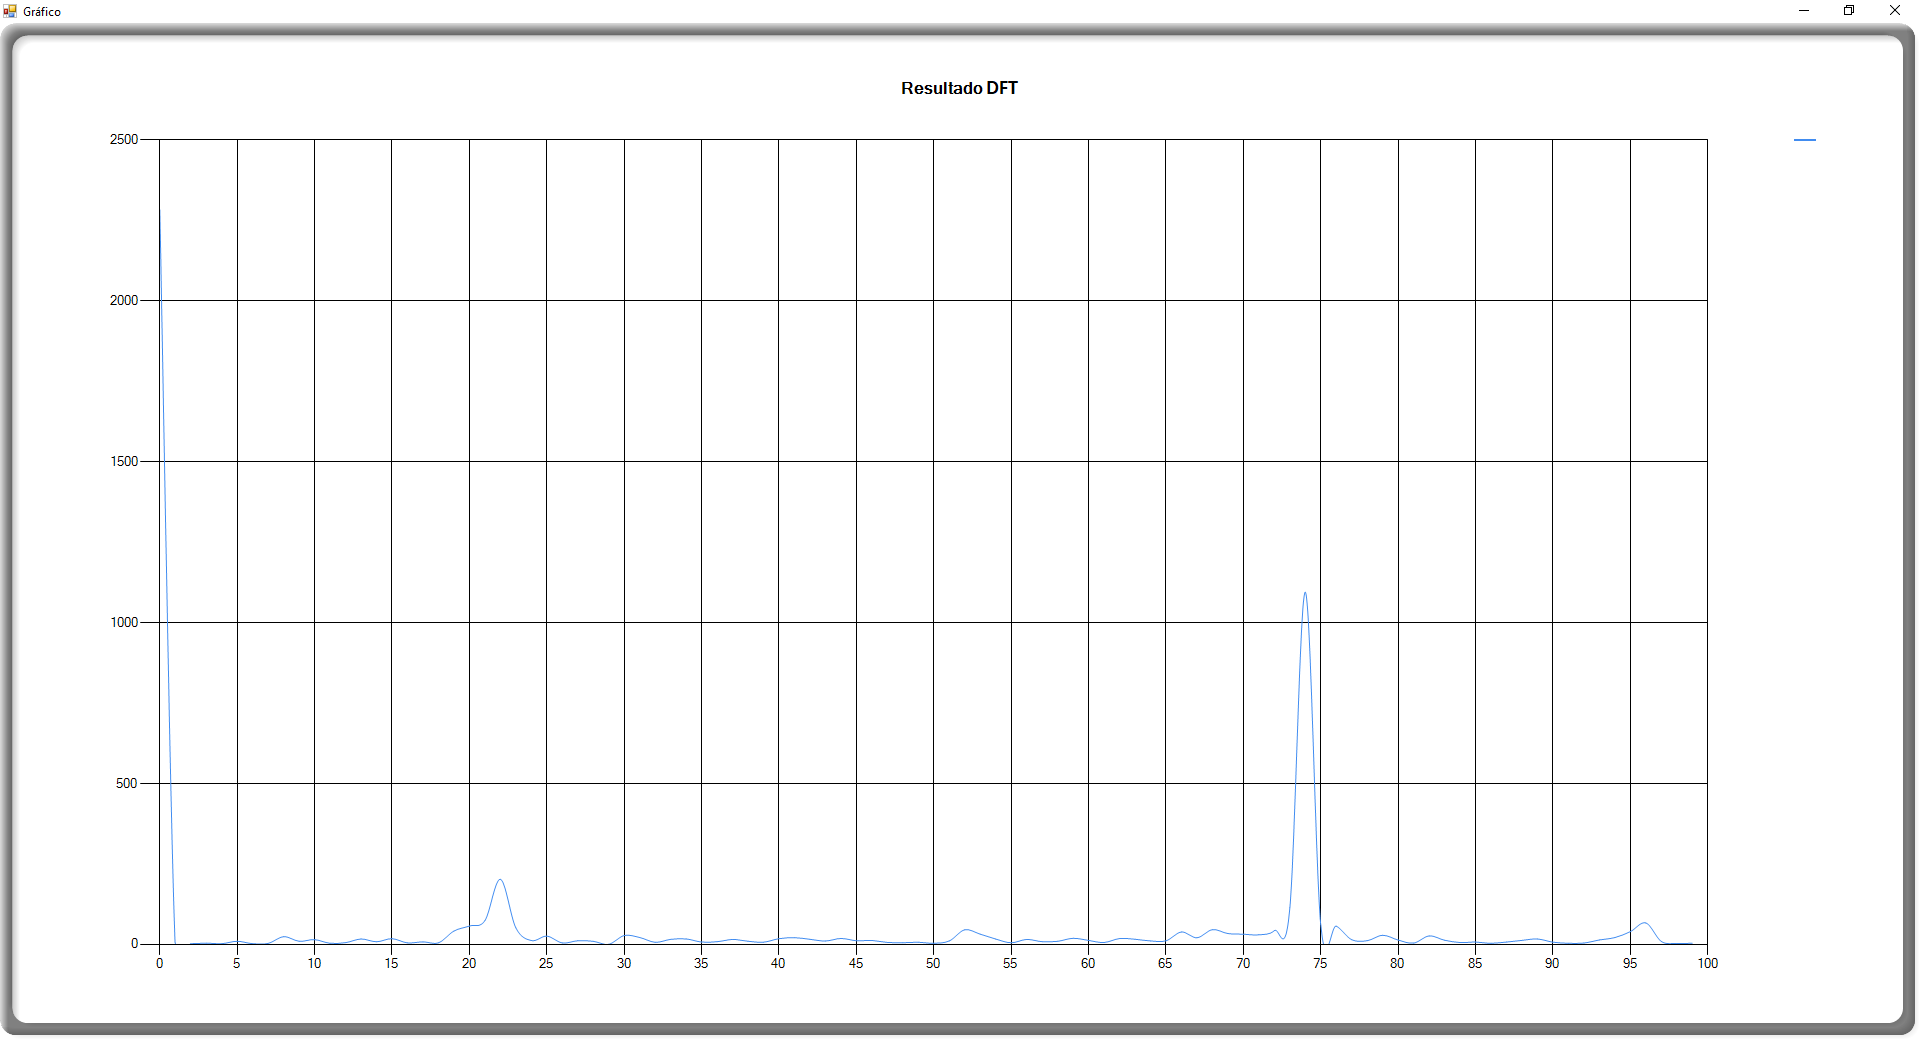
\includegraphics[scale=0.37]{figuras/dft67}
	}
	\fonte{os autores.}
\end{figure}

Nas figuras podemos verificar que na DFT houve uma pequena oscilação na frequência do sinal, foram realizado testes com o osciloscópio na saída do hardware e foi constatado que a frequência do mesmo estava correta. Presume-se que pode estar ocorrendo alguma inconsistência no cálculo da DFT no software gerando este deslocamento na frequência do sinal. 



%CONCLUSÃO
\chapter{CONCLUSÃO}
Com o desenvolvimento deste projeto, foi possível praticar os ensinamentos obtidos durante as aulas de instrumentação e processamento de sinais, através da implementação dos filtros e amplificador, juntamente com processamento do sinal em hardware, bem como realizar a análise do sinal em software.
Com isso, os acadêmicos conseguiram compreender e aplicar na prática a teoria vista em sala de aula, também possibilitou realizar tarefas em equipe, aprendendo a administrar conflitos, melhorar comunicação, ter paciência, entre outros quesitos para um ambiente agradável.

% ----------------------------------------------------------
% ELEMENTOS PÓS-TEXTUAIS
% ----------------------------------------------------------
\postextual

% ----------------------------------------------------------
% Referências bibliográficas
% ----------------------------------------------------------

\bibliography{referencias}

%Apêndices
\begin{apendicesenv}
	
\chapter*{Apêndice A - Código fonte do Firmware}

\begin{lstlisting}[style=CPP]
#include <xc.h>
#include <stdlib.h>
#include <math.h>

#define _XTAL_FREQ	   20000000 
#pragma config FOSC  = HS   
#pragma config WDTE  = OFF  	
#pragma config PWRTE = ON   	
#pragma config BOREN = OFF		
#pragma config LVP   = OFF  	
#pragma config CPD   = OFF  	
#pragma config CP    = OFF  	

unsigned short ADCResult = 0;
int picos = 0, flag = 0;

void USARTInit(long BaudRate, int Mode)
{
int BR = 0;


if (Mode == 0)		
{
BR = (_XTAL_FREQ / (64 * BaudRate)) - 1;
SPBRG = BR;
}
else				
{
BR = (_XTAL_FREQ / (16 * BaudRate)) - 1;
SPBRG = BR;
}


TXSTAbits.CSRC	= 1;	
TXSTAbits.TX9	= 0;	
TXSTAbits.TXEN	= 1; 	
TXSTAbits.SYNC	= 0; 
TXSTAbits.BRGH	= Mode;	
TXSTAbits.TRMT	= 1;	
TXSTAbits.TX9D	= 0;	


RCSTAbits.SPEN	= 1;	
RCSTAbits.RX9	= 0;   
RCSTAbits.SREN	= 0;	
RCSTAbits.CREN	= 1;   	
RCSTAbits.ADDEN	= 0;  
RCSTAbits.FERR	= 0;	
RCSTAbits.OERR	= 0;	
RCSTAbits.RX9D	= 0;	

PIE1bits.RCIE 	= 1;
PIR1bits.RCIF 	= 0;	
}

void USARTWriteChar(unsigned char USARTData)
{
while(!PIR1bits.TXIF);
TXREG = USARTData;
}


void USARTWriteString(const char *str)
{

while(*str != '\0')
{

USARTWriteChar(*str);
str++;
}
}


void ADCInit()
{

ADCON1bits.ADFM 	= 1;	


ADCON1bits.PCFG3 	= 0;	
ADCON1bits.PCFG2 	= 0;	
ADCON1bits.PCFG1 	= 0;	
ADCON1bits.PCFG0 	= 0;	

ADCON0bits.ADCS1 	= 1;	
ADCON0bits.ADCS0 	= 0;	

ADCON0bits.CHS2		= 1;	
ADCON0bits.CHS1		= 0;	
ADCON0bits.CHS0		= 1;	

ADCON0bits.ADON		= 1;


PIE1bits.ADIE 		= 1;	
PIR1bits.ADIF 		= 0;	/	
}


void ADCRead()
{

__delay_us(25); 		
ADCON0bits.GO = 1;			
while(ADCON0bits.GO_DONE);	
}


void TMRInit(){

T1CONbits.T1OSCEN = 0;
T1CONbits.T1CKPS1 = 1; 
T1CONbits.T1CKPS0 = 1;
T1CONbits.TMR1ON = 1;
PIE1bits.TMR1IE = 1;

}

void interrupt ISR(void)
{

if (PIR1bits.TMR1IF)
{		

TMR1 = 62411;	

ADCRead();  
PIR1bits.TMR1IF = 0; 
}

if (PIR1bits.ADIF)
{	
ADCResult = ((ADRESH << 8) + ADRESL);


char * buf;
float input;
int status;

input = ADCResult * 0.0048828125; 
buf = ftoa(input, &status);	 
USARTWriteString("[");
USARTWriteString(buf);
USARTWriteString("]");

PIR1bits.ADIF = 0;	
}
}

void main(void)
{
TRISB	= 0x00;			
PORTB	= 0; 	
TRISC	= 0x80;			
PORTC	= 0;  				
TRISD	= 0x00;			
PORTD	= 0;	
TRISE	= 0xFF;			
PORTE	= 0;  				

TMRInit();				
USARTInit(110000,1);	
ADCInit();			

INTCONbits.PEIE	= 1;	
INTCONbits.GIE	= 1;	
while(1)			
{		

}
}	
\end{lstlisting}

	

\chapter*{Apêndice B - Código fonte do Software Supervisório}

\begin{lstlisting}[language={[Sharp]C}]
namespace SupervisorioInstrumentacao
{
using System;
using System.Collections.Generic;
using System.IO;
using System.IO.Ports;
using System.Threading;
using System.Windows.Forms;

public partial class FrmPrincipal : Form
{
#region Campos

private List<byte> listaBytes;

private List<double> listaDouble;

private List<string> listaString;

private List<char> listaChar;

private List<double> listaDoubleDft;
#endregion

#region Propriedades

private string StringRx { get; set; }


private List<byte> ListaBytes
{
get
{
if (this.listaBytes == null)
{
this.listaBytes = new List<byte>();
}

return this.listaBytes;
}
}

private List<string> ListaString
{
get
{
if (this.listaString == null)
{
this.listaString = new List<string>();
}

return this.listaString;
}
}

private List<char> ListaChar
{
get
{
if (this.listaChar == null)
{
this.listaChar = new List<char>();
}

return this.listaChar;
}
}

private List<double> ListaDouble
{
get
{
if (this.listaDouble == null)
{
this.listaDouble = new List<double>();
}

return this.listaDouble;
}
}

private List<double> ListaDoubleDft
{
get
{
if (this.listaDoubleDft == null)
{
this.listaDoubleDft = new List<double>();
}

return this.listaDoubleDft;
}
}

private DateTime TerminoLeituraDados { get; set; }
#endregion

#region Construtor

public FrmPrincipal()
{
this.InitializeComponent();

this.CarregarListaPortas();


this.cmbVelocidade.SelectedIndex = 0;
this.AlterarEstadoComponentes();

this.btnAnalisar.Enabled = this.ListaDouble.Count > 0;
this.btnCalcularDft.Enabled = this.ListaDouble.Count > 0;
}
#endregion

#region Metodos
#region Componentes do Form

private void btnRecarregarPortas_Click(object sender, EventArgs e)
{
this.CarregarListaPortas();
}

private void btnConectar_Click(object sender, EventArgs e)
{
try
{
if ((this.cmbPortas.SelectedItem == null) ||
string.IsNullOrEmpty(this.cmbPortas.SelectedItem.ToString()))
{
throw new Exception("A porta selecionada e invalida.");
}

this.Conexao.ReadBufferSize = 20000;
this.Conexao.WriteBufferSize = 20000;
this.Conexao.PortName = this.cmbPortas.SelectedItem.ToString();
this.Conexao.BaudRate = int.Parse(this.cmbVelocidade.SelectedItem.ToString());
this.Conexao.Open();
this.Conexao.DiscardInBuffer();
this.txtResultadoSerial.AppendText("Conectado com Sucesso" + Environment.NewLine);


this.ListaBytes.Clear();
this.ListaChar.Clear();
this.ListaDouble.Clear();
this.Conexao.DiscardInBuffer();

int contador = 0;
do
{
contador = this.Conexao.BytesToRead;
} while (contador < 10000);

int byteCount = this.Conexao.BytesToRead;

char[] buffer = new char[byteCount];


int readBytes = this.Conexao.Read(buffer, 0, byteCount);

this.ListaChar.AddRange(buffer);


this.txtResultadoSerial.AppendText("Enviado: #P" + Environment.NewLine);
this.Conexao.Write("#P");
this.Conexao.Close();

this.txtResultadoSerial.AppendText("Serial Parada." + Environment.NewLine);


this.TratarDados();
}
catch (Exception ex)
{
MessageBox.Show(
string.Format(
"[Erro]{1}{0}{1}{1}[StackTrace]{1}{2}{1} Porta: {3}{1} Velocidade: {4}",
ex.Message,
Environment.NewLine,
ex.StackTrace,
this.cmbPortas.SelectedItem == null ? "Nulo" : this.cmbPortas.SelectedItem.ToString(),
this.cmbVelocidade.SelectedItem == null ? "Nulo" : this.cmbVelocidade.SelectedItem.ToString()),
"Erro",
MessageBoxButtons.OK,
MessageBoxIcon.Error);
}
}

private void btnAnalisar_Click(object sender, EventArgs e)
{

FrmChart frmChart = new FrmChart(this.ListaDouble, "Dados Recebidos");
frmChart.ShowDialog();
}

private void btnApresentarDft_Click(object sender, EventArgs e)
{

FrmChart frmChart = new FrmChart(this.ListaDoubleDft, "Resultado DFT");
frmChart.ShowDialog();
}

private void btnCalcularDft_Click(object sender, EventArgs e)
{
try
{
this.CalcularDft(200, 'l');

this.txtResultadoSerial.AppendText("Calculo OK." + Environment.NewLine);
}
catch (Exception ex)
{
MessageBox.Show(
string.Format(
"[Erro]{1}{0}{1}{1}[StackTrace]{1}{2}{1} Porta: {3}{1} Velocidade: {4}",
ex.Message,
Environment.NewLine,
ex.StackTrace,
this.cmbPortas.SelectedItem == null ? "Nulo" : this.cmbPortas.SelectedItem.ToString(),
this.cmbVelocidade.SelectedItem == null ? "Nulo" : this.cmbVelocidade.SelectedItem.ToString()),
"Erro",
MessageBoxButtons.OK,
MessageBoxIcon.Error);
}
}
#endregion

#region Privados

private void CarregarListaPortas()
{
try
{

string portaConectada = string.Empty;
if (this.cmbPortas.SelectedValue != null)
{
portaConectada = this.cmbPortas.SelectedValue.ToString();
}

this.cmbPortas.Items.Clear();

string[] ports = SerialPort.GetPortNames();
foreach (string port in ports)
{
int convert = 0;
if (!int.TryParse(port.Substring(3), out convert))
{
continue;
}

this.cmbPortas.Items.Add("COM" + convert.ToString());
}

for (int i = 0; i < this.cmbPortas.Items.Count; i++)
{
if (this.cmbPortas.Items[i].ToString() == portaConectada)
{
this.cmbPortas.SelectedIndex = i;
}
}

this.AlterarEstadoComponentes();
}
catch (Exception ex)
{
MessageBox.Show(
string.Format(
"Ocorreu o seguinte erro ao atualizar as portas:{0}[Erro]{1}{0}Tente novamente.",
Environment.NewLine,
ex.Message),
"Erro",
MessageBoxButtons.OK,
MessageBoxIcon.Error);
}
}

private void AlterarEstadoComponentes()
{
try
{

this.cmbPortas.Enabled = this.cmbPortas.Items.Count > 0;
this.btnConectar.Enabled = this.cmbPortas.Items.Count > 0;
if ((this.cmbPortas.Items.Count > 0) && (this.cmbPortas.SelectedValue == null))
{
this.cmbPortas.SelectedIndex = 0;
}
}
catch (Exception ex)
{
MessageBox.Show(
string.Format(
"Ocorreu o seguinte erro ao atualizar os componentes:{0}[Erro]{1}{0}",
Environment.NewLine,
ex.Message),
"Erro",
MessageBoxButtons.OK,
MessageBoxIcon.Error);
}
}

private void AlteraTxtResultado(object sender, EventArgs e)
{
this.txtResultadoSerial.AppendText(string.Format("Dados: {0}{1}", this.StringRx, Environment.NewLine));
}

private void TratarDados()
{

this.txtResultadoSerial.AppendText("Iniciando o tratamento dos dados." + Environment.NewLine);

string resultado = string.Empty;
foreach (char teste in this.ListaChar)
{
if (teste == '[')
{
resultado = string.Empty;
continue;
}

if (teste == ']')
{
this.ListaDouble.Add(Convert.ToDouble(resultado.Replace('.', ',')));
continue;
}

resultado += teste;
}

this.btnAnalisar.Enabled = this.ListaDouble.Count > 0;
this.btnCalcularDft.Enabled = this.ListaDouble.Count > 0;

}

private void CalcularDft(double frequenciaAmostragem, char tipo)
{
 
double somaR = 0;
double somaI = 0;
double mag = 0;
double N = 0;
int k = 0;
int n = 0;


N = frequenciaAmostragem / 2.0;

this.ListaDoubleDft.Clear();
for (k = 0; k < N; k++)
{
somaR = 0;
somaI = 0;

for (n = 0; n < (int)this.ListaDouble.Count; n++)
{
somaR = somaR + this.ListaDouble[n] * Math.Cos((2.0 * Math.PI / frequenciaAmostragem) * k * n);
somaI = somaI - this.ListaDouble[n] * Math.Sin((2.0 * Math.PI / frequenciaAmostragem) * k * n);
}


mag = Math.Sqrt(Math.Pow(somaR, 2) + Math.Pow(somaI, 2));


switch (tipo)
{
case 'd':
this.ListaDoubleDft.Add(20 * Math.Log10(mag));
break;

case 'l':
this.ListaDoubleDft.Add(mag);
break;
}
}

this.btnApresentarDft.Enabled = this.ListaDoubleDft.Count > 0;
}
#endregion
#endregion
}
}
\end{lstlisting}



\end{apendicesenv}




%Anexos
%\begin{anexosenv}
\chapter*{Título do Anexo A}

\lipsum[1-1]


\end{anexosenv}

%---------------------------------------------------------------------
% INDICE REMISSIVO
%---------------------------------------------------------------------

\printindex
\end{document}